\documentclass[tikz,border=3mm,multi=tikzpicture]{standalone}
\usepackage[utf8]{inputenc}
\usepackage[T1]{fontenc}
\usepackage{helvet}
\renewcommand{\familydefault}{\sfdefault}
\usepackage{tikz}
\usetikzlibrary{arrows.meta}
\begin{document}

\tikzset{every node/.append style={font=\sffamily\small}}
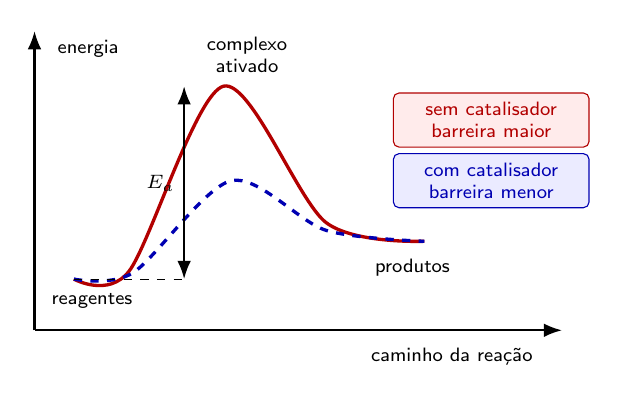
\begin{tikzpicture}[x=1cm,y=1cm,>=Latex,
  every node/.append style={font=\sffamily\scriptsize}]
  \draw[->,thick] (0.45,0.45) -- (7.15,0.45);
  \node[align=center] at (5.75,0.12) {caminho da reação};
  \draw[->,thick] (0.45,0.45) -- (0.45,4.25);
  \node[anchor=west] at (0.62,4.02) {energia};

  \draw[very thick,red!70!black] plot[smooth] coordinates {(0.95,1.1) (1.65,1.2) (2.85,3.55) (4.15,1.82) (5.4,1.58)};
  \draw[very thick,blue!70!black,dashed] plot[smooth] coordinates {(0.95,1.1) (1.7,1.18) (2.95,2.35) (4.15,1.72) (5.4,1.58)};

  \draw[dashed] (0.95,1.1) -- (2.35,1.1);
  \draw[<->,thick] (2.35,1.1) -- (2.35,3.55);
  \node[align=center] at (2.05,2.32) {$E_a$};

  \node[align=center] at (3.15,3.95) {complexo\\ativado};
  \node[align=center] at (1.18,0.82) {reagentes};
  \node[align=center] at (5.25,1.25) {produtos};

  \node[draw=red!70!black,rounded corners=2pt,fill=red!8,text=red!70!black,align=center,text width=2.25cm] at (6.25,3.12)
    {sem catalisador\\barreira maior};
  \node[draw=blue!70!black,rounded corners=2pt,fill=blue!8,text=blue!70!black,align=center,text width=2.25cm] at (6.25,2.35)
    {com catalisador\\barreira menor};
\end{tikzpicture}

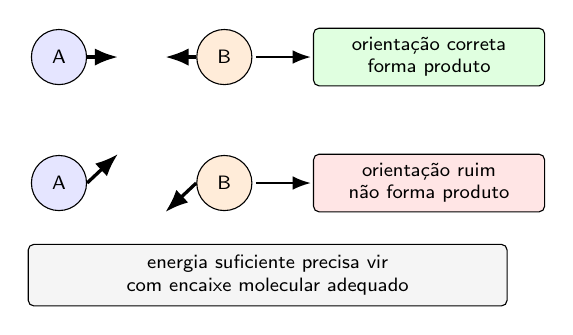
\begin{tikzpicture}[x=1cm,y=1cm,>=Latex,
  every node/.append style={font=\sffamily\scriptsize},
  card/.style={draw,rounded corners=2pt,align=center,text width=2.7cm,minimum height=0.72cm}]
  \node[draw,circle,fill=blue!10,minimum size=0.7cm] (a1) at (0.35,2.15) {A};
  \node[draw,circle,fill=orange!15,minimum size=0.7cm] (b1) at (2.45,2.15) {B};
  \draw[->,very thick] (a1.east) -- (1.1,2.15);
  \draw[->,very thick] (b1.west) -- (1.7,2.15);
  \draw[->,thick] (2.85,2.15) -- (3.55,2.15);
  \node[card,fill=green!12] at (5.05,2.15) {orientação correta\\forma produto};

  \node[draw,circle,fill=blue!10,minimum size=0.7cm] (a2) at (0.35,0.55) {A};
  \node[draw,circle,fill=orange!15,minimum size=0.7cm] (b2) at (2.45,0.55) {B};
  \draw[->,very thick] (a2.east) -- (1.1,0.92);
  \draw[->,very thick] (b2.west) -- (1.7,0.18);
  \draw[->,thick] (2.85,0.55) -- (3.55,0.55);
  \node[card,fill=red!10] at (5.05,0.55) {orientação ruim\\não forma produto};

  \node[draw,rounded corners=2pt,fill=gray!8,align=center,text width=5.8cm,inner sep=4pt] at (3.0,-0.62)
    {energia suficiente precisa vir\\com encaixe molecular adequado};
\end{tikzpicture}
\end{document}
